\def\year{2020}\relax
%File: formatting-instruction.tex
\documentclass[letterpaper]{article} % DO NOT CHANGE THIS
\usepackage{aaai20}  % DO NOT CHANGE THIS
\usepackage{times}  % DO NOT CHANGE THIS
\usepackage{helvet} % DO NOT CHANGE THIS
\usepackage{courier}  % DO NOT CHANGE THIS
\usepackage[hyphens]{url}  % DO NOT CHANGE THIS
\usepackage{graphicx} % DO NOT CHANGE THIS
\usepackage{subcaption}
\urlstyle{rm} % DO NOT CHANGE THIS
\def\UrlFont{\rm}  % DO NOT CHANGE THIS
\usepackage{graphicx}  % DO NOT CHANGE THIS
\frenchspacing  % DO NOT CHANGE THIS
\setlength{\pdfpagewidth}{8.5in}  % DO NOT CHANGE THIS
\setlength{\pdfpageheight}{11in}  % DO NOT CHANGE THIS
%\nocopyright
%PDF Info Is REQUIRED.
% For /Author, add all authors within the parentheses, separated by commas. No accents or commands.
% For /Title, add Title in Mixed Case. No accents or commands. Retain the parentheses.
 \pdfinfo{
/Title (Maximização de pontuação no jogo Freeway utilizando os algoritmos de aprendizado por reforço Proximal Policy Optimization (PPO) e Deep Q-Learning (DQN))
/Author (Vinicius Alves Matias)
} %Leave this	
% /Title ()
% Put your actual complete title (no codes, scripts, shortcuts, or LaTeX commands) within the parentheses in mixed case
% Leave the space between \Title and the beginning parenthesis alone
% /Author ()
% Put your actual complete list of authors (no codes, scripts, shortcuts, or LaTeX commands) within the parentheses in mixed case. 
% Each author should be only by a comma. If the name contains accents, remove them. If there are any LaTeX commands, 
% remove them. 

% DISALLOWED PACKAGES
% \usepackage{authblk} -- This package is specifically forbidden
% \usepackage{balance} -- This package is specifically forbidden
% \usepackage{caption} -- This package is specifically forbidden
% \usepackage{color (if used in text)
% \usepackage{CJK} -- This package is specifically forbidden
% \usepackage{float} -- This package is specifically forbidden
% \usepackage{flushend} -- This package is specifically forbidden
% \usepackage{fontenc} -- This package is specifically forbidden
% \usepackage{fullpage} -- This package is specifically forbidden
% \usepackage{geometry} -- This package is specifically forbidden
% \usepackage{grffile} -- This package is specifically forbidden
% \usepackage{hyperref} -- This package is specifically forbidden
% \usepackage{navigator} -- This package is specifically forbidden
% (or any other package that embeds links such as navigator or hyperref)
% \indentfirst} -- This package is specifically forbidden
% \layout} -- This package is specifically forbidden
% \multicol} -- This package is specifically forbidden
% \nameref} -- This package is specifically forbidden
% \natbib} -- This package is specifically forbidden -- use the following workaround:
% \usepackage{savetrees} -- This package is specifically forbidden
% \usepackage{setspace} -- This package is specifically forbidden
% \usepackage{stfloats} -- This package is specifically forbidden
% \usepackage{tabu} -- This package is specifically forbidden
% \usepackage{titlesec} -- This package is specifically forbidden
% \usepackage{tocbibind} -- This package is specifically forbidden
% \usepackage{ulem} -- This package is specifically forbidden
% \usepackage{wrapfig} -- This package is specifically forbidden
% DISALLOWED COMMANDS
% \nocopyright -- Your paper will not be published if you use this command
% \addtolength -- This command may not be used
% \balance -- This command may not be used
% \baselinestretch -- Your paper will not be published if you use this command
% \clearpage -- No page breaks of any kind may be used for the final version of your paper
% \columnsep -- This command may not be used
% \newpage -- No page breaks of any kind may be used for the final version of your paper
% \pagebreak -- No page breaks of any kind may be used for the final version of your paperr
% \pagestyle -- This command may not be used
% \tiny -- This is not an acceptable font size.
% \vspace{- -- No negative value may be used in proximity of a caption, figure, table, section, subsection, subsubsection, or reference
% \vskip{- -- No negative value may be used to alter spacing above or below a caption, figure, table, section, subsection, subsubsection, or reference

\setcounter{secnumdepth}{0} %May be changed to 1 or 2 if section numbers are desired.

% The file aaai20.sty is the style file for AAAI Press 
% proceedings, working notes, and technical reports.
%
\setlength\titlebox{2.5in} % If your paper contains an overfull \vbox too high warning at the beginning of the document, use this
% command to correct it. You may not alter the value below 2.5 in
\title{Maximização de pontuação no jogo Freeway através de Aprendizado por Reforço}
%Your title must be in mixed case, not sentence case. 
% That means all verbs (including short verbs like be, is, using,and go), 
% nouns, adverbs, adjectives should be capitalized, including both words in hyphenated terms, while
% articles, conjunctions, and prepositions are lower case unless they
% directly follow a colon or long dash
\author{Vinicius Alves Matias\textsuperscript{\rm 1} \\ 
\textsuperscript{\rm 1}Escola de Artes, Ciências e Humanidades da Universidade de São Paulo\\ %If you have multiple authors and multiple affiliations
% use superscripts in text and roman font to identify them. For example, Sunil Issar,\textsuperscript{\rm 2} J. Scott Penberthy\textsuperscript{\rm 3} George Ferguson,\textsuperscript{\rm 4} Hans Guesgen\textsuperscript{\rm 5}. Note that the comma should be placed BEFORE the superscript for optimum readability
Rua Arlindo Bettio, 1000, São Paulo/SP\\
viniciusmatias@usp.br % email address must be in roman text type, not monospace or sans serif
}

 \begin{document}

\maketitle

\begin{abstract}
Algoritmos de Aprendizado por reforço têm diversas aplicações na literatura, mas um tópico extremamente interessante é a utilização de jogos para avaliação do desempenho dos algoritmos. A utilização de games do  Atari em um ambiente controlado podem servir de base para o estudo da generalização de algoritmos em inteligência artificial. Neste relatório será discutida a aplicação de dois algoritmos relativamente recentes (menos de 10 anos da primeira publicação), mas que em muitos casos permitem que um agente aprenda em uma ambiente qualquer sem nenhuma grande adaptação ao método original proposto. Os algoritmos de Aprendizado por Reforço analisados foram o Proximal Policy Optimation (PPO) e o Deep Q-Learning Network (DQN). Para uma análise em um ambiente discretizado foram usados os algoritmos Value Iteration (VI) e Policy Iteration (PI). O jogo do Atari escolhido foi o Freeway, tendo este um ponto específico de recompensas esparsas. 
\end{abstract}

\section{Introdução}
Freeway é um jogo desenvolvido pela Activision e disponibilizado no Atari 2600 (Activision 1981). O objetivo do jogo é fazer uma galinha atravessar uma via expressa enquanto desvia de veículos, acumulando um ponto ao atravessar todas as faixas sem ser atingida. A pontuação máxima possível é igual à 34 pontos. Quando a galinha encontra um carro, ela volta duas posições com um delay curto, podendo ser atingida por outros carros nesse período. A interface do game que será usado no projeto pode ser vista na figura 1.

\begin{figure}[h]
\centering
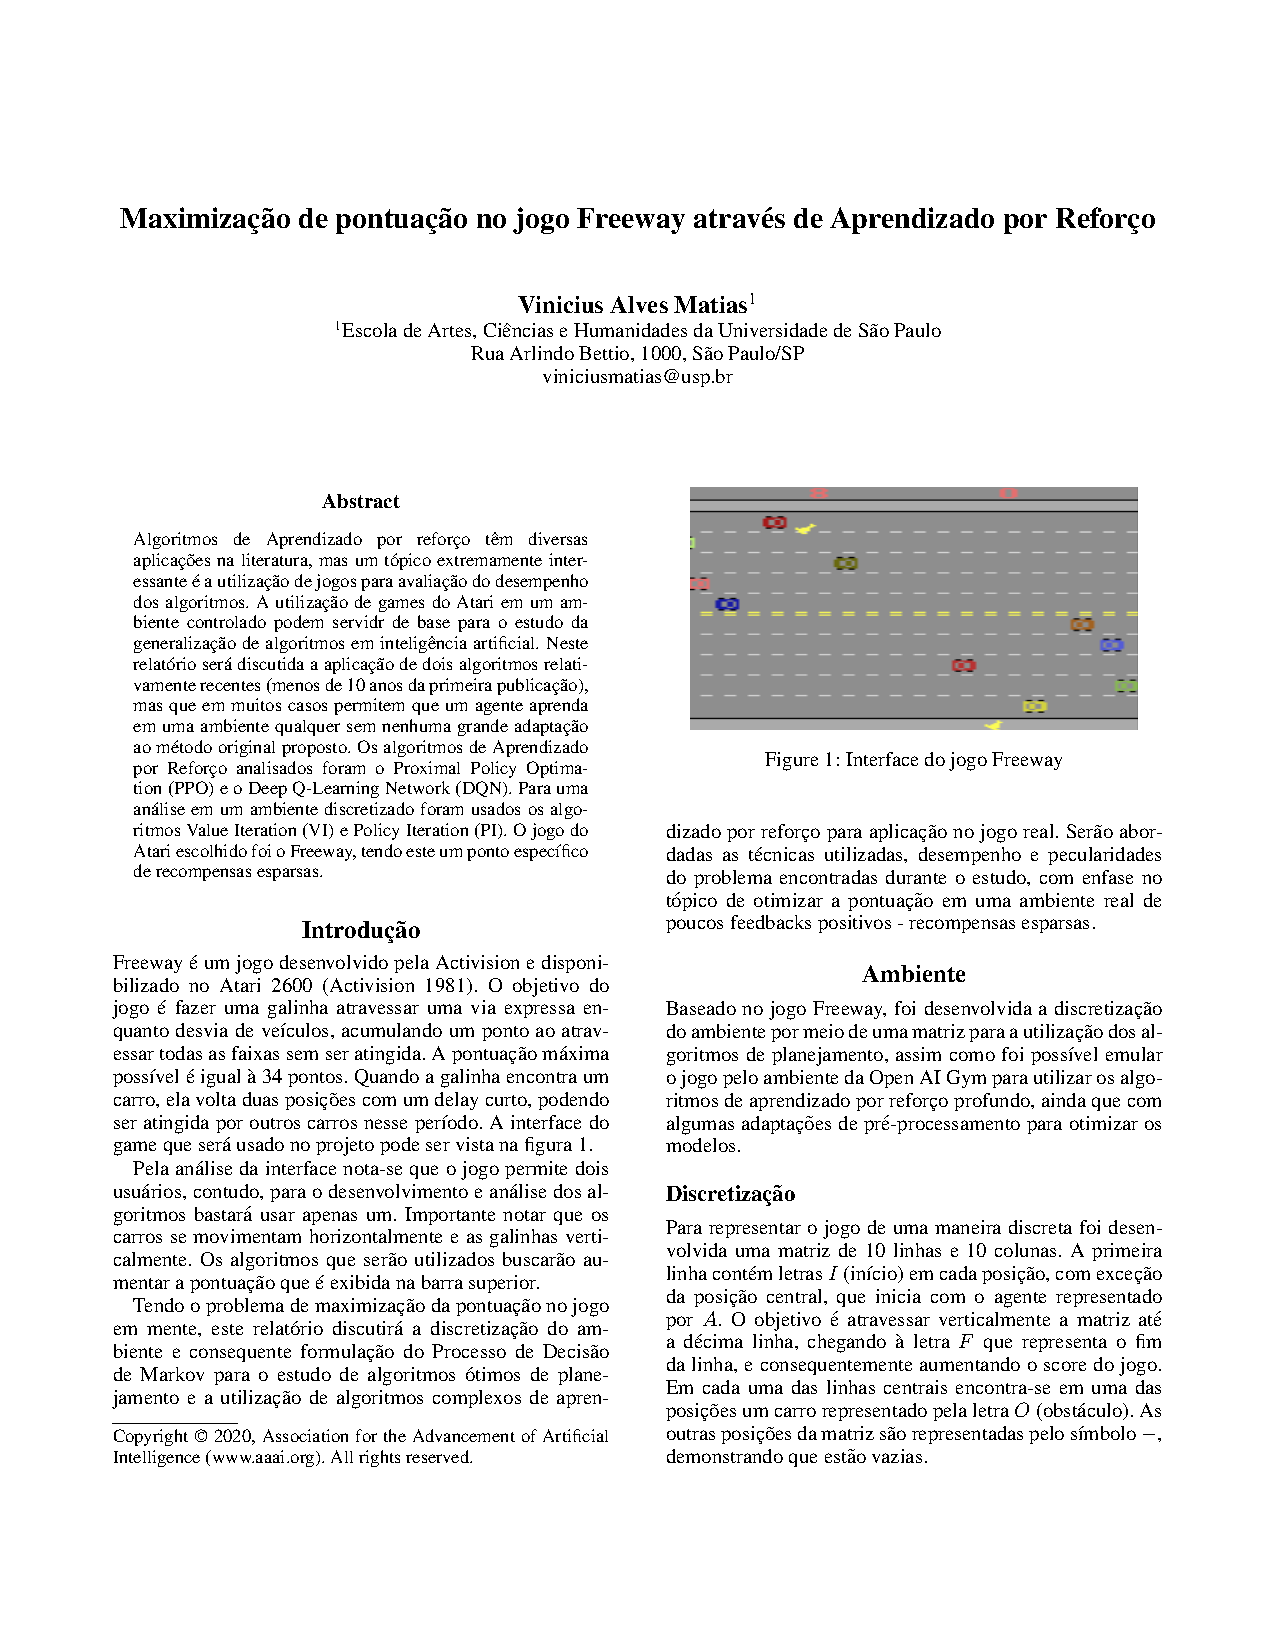
\includegraphics[width=0.9\columnwidth]{freeway}
\caption{Interface do jogo Freeway}
\label{freeway}
\end{figure}

Pela análise da interface nota-se que o jogo permite dois usuários, contudo, para o desenvolvimento e análise dos algoritmos bastará usar apenas um. Importante notar que os carros se movimentam horizontalmente e as galinhas verticalmente. Os algoritmos que serão utilizados buscarão aumentar a pontuação que é exibida na barra superior.

Tendo o problema de maximização da pontuação no jogo em mente, este relatório discutirá a discretização do ambiente e consequente formulação do Processo de Decisão de Markov para o estudo de algoritmos ótimos de planejamento e a utilização de algoritmos complexos de aprendizado por reforço para aplicação no jogo real \footnote{Códigos disponíveis em: https://github.com/matiasvinicius/Planning-and-Reinforcement-Learning}. Serão abordadas as técnicas utilizadas, desempenho e pecularidades do problema encontradas durante o estudo, com ênfase no tópico de otimizar a pontuação em uma ambiente real de poucos feedbacks positivos - recompensas esparsas.

\section{Ambiente}
Baseado no jogo Freeway, foi desenvolvida a discretização do ambiente por meio de uma matriz para a utilização dos algoritmos de planejamento, assim como foi possível emular o jogo pelo ambiente da Open AI Gym (Brockamn et al 2016) para utilizar os algoritmos de aprendizado por reforço profundo, ainda que com algumas adaptações de pré-processamento para otimizar os modelos.

\subsection{Discretização}
Para representar o jogo de uma maneira discreta foi desenvolvida uma matriz de 10 linhas e 9 colunas. A primeira linha contém letras $I$ (início) em cada posição, com exceção da posição central, que inicia com o agente representado por $A$. O objetivo é atravessar verticalmente a matriz até a décima linha, chegando à letra $F$ que representa o fim da linha, e consequentemente aumentando o score do jogo. Em cada uma das linhas centrais encontra-se em uma das posições um carro representado pela letra $O$ (obstáculo), inserido de forma aleatória. As outras posições da matriz são representadas pelo símbolo $-$, demonstrando que estão vazias. 

Como o jogo tem um tempo limite de 136 segundos, o ambiente também terá um tempo delimitado especificado. Para este artigo seguimos que existirão 272 iterações (uma referência à possibilidade ocorrem duas mudanças no ambiente por segundo), isto é, para cada iteração $t$ o agente poderá tomar uma ação, assim como os carros se moverão para a próxima posição válida na sua linha - à direita ou na primeira posição à esquerda quando chega ao limite do campo. Para o ambiente discreto não foi considerada uma velocidade específica para cada veículo, mas sim uma mesma para todos. A figura 2 exemplifica essa mudança do ambiente para uma próxima iteração.

\begin{figure}[h]
     \begin{subfigure}[h]{0.2\textwidth}
         \centering
         \includegraphics[width=\textwidth]{discreto_t1.png}
         \caption{Ambiente em $t$}
     \end{subfigure}
     \hfill
     \begin{subfigure}[h]{0.2\textwidth}
         \includegraphics[width=\textwidth]{discreto_t2.png}
         \caption{Ambiente em $t+1$}
     \end{subfigure}
        \caption{Matriz que representa o ambiente discreto em um momento $t$ (a) e $t+1$ (b)}
\end{figure}

A maneira que permite que esse ambiente funcione de forma não dinâmica para a aplicação dos algoritmos serão melhor esclarecidos no subtópico de Planejamento Probabilístico \textit{Value Iteration}

\subsection{Pré-Processamento no Atari}
Pelo ambiente de emulação do Atari (Bellemare et al 2013), a velocidade para execução de algoritmos que têm relação à redes neurais muitas vezes é dependente da entrada recebida. Para otimizar os algoritmo DQN foi realizado um redimensionamento nos frames enviados aos jogos. A dimensão de 210px (altura) por 160px (largura) passou para 84X84. Esse redimensionamento influenciou em mais agilidade para realizar os testes, visto que para o DQN (que será visto logo) sem nenhuma adaptação da imagem resultou uma rede neural com mais de 34 milhões de parâmetros possíveis, enquanto a adaptação resultou em cerca de 5 milhões de pesos possíveis. Para este momento do projeto não foram realizadas outras adaptações como na luminância, ajustes para escala de cinza ou junção de dimensões da imagem em um único canal, mencionados no artigo que propos o DQN. Para o PPO, visto que não conseguiu-se até o momento um resultado satisfatório, foi adicionada a mudança na escala de cores do jogo para uma escala de cinza.

\subsection{Recompensas esparsas}
Em planejamento, quando discretizamos o ambiente podemos facilmente determinar recompensas para incentivar o aprendizado de um agente. Isso implica que não teremos apenas recompensas positivas, mas também negativas facilmente detectáveis (chegar ao fim do trajeto é algo positivo e ser atingido por um obstáculo é negativo).

Em ambientes reais, contudo, a definição das recompensas deve estar atrelada ao que se tem disponível do ambiente, não sendo viável reallizar processamentos à mais para adicionar outros tipos de recompensas (como uma definição prévia de processamento para identificar veículos e então atualizá-los como recompensas negativas). Além de aumentar a complexidade do método, processamentos adicionais se afastariam da tentativa de um algoritmo de aprendizado por reforço aprender sem nenhuma interferência externa. Ambientes desse tipo se enquadram no problema de recompensas esparsas, pois o ambiente não é capaz de prover recompensas de maneira acessível ao agente de maneira frequente (Hare 2019).

Isso leva à notar que nosso problema terá apenas uma recompensa bem definida à priori, que é chegar ao fim da via expressa (aumentar o score do jogo). Para adquirir essa recompensa, contudo, o agente deve passar por todos os obstáculos e então receber o feedback.

Isso não é tão incomum em jogos do Atari, tanto que os algoritmos PPO e DQN tentam contornar esses problemas por intermédio da "janela" (buffer) que terão acesso para definir as melhores ações para um problema. O DQN em especial tem algo que apoia muitos algoritmos no caso de recompensas esparsas: o fato de ser \textit{off-policy}, logo, ainda que busque a ação que otimize a recompensa em um estado, há uma probabilidade de desvirtuar dessa suposta melhor recompensa e, eventualmente, tornar o processo mais eficiente.

É importante notar que ainda que para o \textit{Freeway} as recompensas esparsas não sejam problemas muito grandes por haver um bom tratamento delas, em alguns problemas pode ser mais interessante buscar algoritmos que buscam explorar muito o ambiente em busca de informações que possam ser úteis posteriormente, isto é, algoritmos que "dirigidos à curiosidade" (Pathak et al. 2017) , que possivelmente teriam desempenho decente sob o jogo em questão.


\section{Planejamento Probabilístico}
O ambiente discretizado mencionado no tópico anterior é a base para a aplicação dos algoritmos de planejamento, que são úteis para analisar o comportamento do problema em um ambiente controlado. Antes de iniciar esse estudo, note que a pontuação máxima para essa versão do jogo não é 34 pontos, pois temos 9 posições possíveis para o agente (chegar ao estado meta implica em retornat à posição inicial) e 272 iterações, assim, a máxima pontuação possível será de $\lceil \frac{272}{9}\rceil = 31$ pontos. Com isto dito, podemos definir o MDP (\textit{Markov Decision Process}). Para este MDP consideramos uma tupla $<S,A,D,T,R>$ (Mausam and Kolobov, 2012), onde: 

\begin{itemize}

\item $s \in S$ são os estados. O agente explora uma sequência de 10 estados e cada um, por sua vez, leva informações coluna adjacente ao agente (de onde vêm os obstáculos). Note que o estado inicial $s_0$ é fixo e há um conjunto de estados metas $G$ (posição final da matriz) em que o agente chega ao fim da via expressa. Havendo então a possibilidade de um agente transitar em 10 estados (não se mantém no estado meta, mas transita para ele), e que cada estado pode ser ocupado por um obstáculo, agente ou espaço nulo com exceção do estado meta (que só pode ser ocupado pela referência de meta) e o estado inicial (que terá ou um agente ou espaço vazio), temos que existem $3^{10} + 1 + 2 = 59052$ composições de estado diferentes;

\item $a \in A$ são as ações, tendo um total de 3 ações possíveis. $A$ é representado como um conjunto $A = \{UP, DOWN, NOOP\}$;

\item $d \in D$ é o tempo (ou época) que ocorre a decisão. Visto que há um limite de tempo para finalizar o jogo igual à 136 segundos (Weiss 2007), $D$ é um conjunto finito (isto é, não poderão ser mapeados estados inifinatamente);

\item $T$ é uma função de transição que mapeia os estado corrente, época e ação em um estado $s_{t+1}$. A transição entre estados segue uma política (que cabe aos algoritmos definirem), mas vale notar que a transição é determinista - não segue uma distribuição de probabilidade para definir qual estado ir;

\item $R$ é uma função de recompensa. Os algoritmos de planejamento entregam uma recompensa positiva igual à 1 para estado meta, -1 para a colisão com os obstáculos, e nula para qualquer outra posição. O estado meta com recompensa +2 foi testado também, mas não trouxe nenhuma grande diferença para várias execuções dos algoritmos (variação de menos de um ponto na pontuação média).

\end{itemize}

Problemas de Horizonte indeterminado englobam o conceito de estados meta, e de fato à um estado que o agente não sabe que deve chegar sem auxílio de um algoritmo. Esse ponto de indeterminação fica muito claro na necessidade de explorar o ambiente na fase de aprendizado por reforço, pois não recebe nenhum retorno positivo até encontrar o que poderia ser definido como meta e aumentar seu \textit{score}. Em planejamento, podemos aproveitar o fato de delimitarmos o limite do processo (estado com recompensa positiva), e executar os algoritmos à partir dele como um algoritmo para Horizonte Finito.

Visto que queremos maximar a pontuação e a formulação do jogo, devemos buscar uma política $\pi$ markoviana (decisão depende apenas do estado inicial em planejamento, apesar de poder se aproveitar de um \textit{buffer} com o histórico, como será visto em aprendizado por reforço), estacionária (não há uma relação entre tempo e transição/recompensa) e determinista (sempre será feita a mesma ação para um mesmo estado).

\subsection{Value Iteration}
A Iteração de Valor (Sutton and Barto 2020) é um método usado em planejamento quando busca-se identificar qual estado de todo seu ambiente discreto é o que terá a melhor "recompensa" total, ou seja, maior valor. O Valor de cada estado é calculado mediante a aplicação do princípio de otimilidade de \textit{Bellman} para a incerteza de um ambiente (O'Donoghue et al 2018). Independente do estado inicial que se aplica a equação de Bellman, este deverá identificar o valor ótimo para o estado em questão. A questão da definição da política ótima é deixada em segundo plano no \textit{Value Iteration}, isto porque, como dito, ele visa retornar o valor de um estado, e não a melhor ação à tomar. A função valor ótima $V^{*}(s, n)$ para um estado $s$ em um passo $n$ de um problema de Horizon Finito é dada por:

$$
V^{*}(s, n) = \max_{a \in A} \ \{ R(s,a) + \sum_{s' \in S} T(s,a,s')  V(s', n-1)\}
$$

Essa equação é aplicada no problema de maneira recursiva à partir do estado meta do ambiente discretizado, e vai calculando o valor de todos os estados mediante a recompensa do estado $s'$ e a probabilidade de alcançá-lo com uma das três ações possíveis.

Como a iteração de valor não retorna uma política, é necessária uma adaptação ao método para, ao final, coletarmos a ação que proporcione o maior resultado para as ações possíveis em um estado $s$, ou seja:

$$
\pi(s, n) = arg \max_{a \in A} \ \{ R(s,a) + \sum_{s' \in S} T(s,a,s')  V(s', n-1)\}
$$

A recorrência permite a convergência do algoritmo à política ótima, mas ainda assim ele depende da definição de um ambiente que possa coletar alguma pontuação, caso contrário, pontuará zero. Esse detalhe é importante pois, como mencionado na discretização do ambiente, os obstáculos são postos em posições aleatórias da matriz, e essa composição pode, em muitos casos, gerar um ambiente cujo agente não consiga chegar ao estado meta visto que cada estado inclui informações apenas da coluna adjacente às posições possíveis para deslocamente, justamente para reduzir a complexidade do método. O exemplo mais extremo desse caso, mas não restrito somente à ele, é de todos os obstáculos entrarem na mesma coluna, implicando que em algum momento o agente colidirá com um obstáculo, e em uma reação de cadeia levará ele de volta ao início. Como sempre há três ações possíveis para o agente, ele escolherá a melhor para o momento, mas no futuro essa ação ótima poderá sofrer influência da constituição do ambiente e levâ-lo de volta ao início de maneira constante. 

Optamos por manter essa composição no ambiente discreto. A Activision, para evitar esse problema, inicializa, em toda a partida, os agentes na mesma posição e com mesma velocidade (portanto, não será um detalhe relevante para a etapa de aprendizado por reforço).

Outro detalhe de ambientes discretos é que eles não devem dinâmicos. Para criar resultados que facilitem a comparação com algoritmos de aprendizado por reforço, utilizamos cada \textit{frame} (instante t do ambiente desenvolvido) como um ambiente discreto, ou seja, uma representação do jogo que pode ter algoritmos de planejamento probabilístico aplicáveis e, portanto, ter uma ação ótima de um estado para outro. A transição de um \textit{frame} para outro implica em mais uma execução do \textit{Value Iteration}. Ao fim são esperadas $n\_epochs * 272$  cálculos do método de iteração de valor. Cada iteração teve em média 300 equações de \textit{Bellman} executadas. Os resutados de 360 jogos podem ser vistos na figura a seguir.

\begin{figure}[h]
	\center
	\includegraphics[width=0.4\textwidth]{value_iteration}
    \caption{Execuções do Value Iteration. Cada "jogo" é composto por 272 iterações de valor seguidas em um ambiente de 10 estados.}
\end{figure}

\begin{figure}[h]
	\center
	\includegraphics[width=0.4\textwidth]{hist_vi}
    \caption{Histograma do Value Iteration.}
\end{figure}


Como explicado neste tópico, o resultado um tanto quanto contra intuitivo de pontuações nulas mostrada na figura tem uma explicação: a aleatoriedade da composição dos ambientes, e a sequência de ações ótima possível não necessariamente resultar em alcançar a meta.

Ainda assim, a maioria das pontuações finais foram de 15 pontos, com a maior densidade nos valores entre 28 e 30 pontos, implicando em uma média de 24.89 pontos. Vale notar que para atingir 31 pontos, os estados de maior valor deveriam sempre estar atrelados à ação de ir para frente, pois essa pontuação só é possível se, durante toda a execução do jogo, for possível ir para frente (após um longo período de treinamento, os algoritmos de aprendizado por reforço apresentam essa mesma tática, de ir sempre que possível à frente, mesmo que colidam com obstáculos e voltem duas casas).

\subsection{Policy Iteration}
O algoritmo \textit{Value Iteration} retorna o valor ótimo para os estados de uma ambiente discreto (no caso, cada \textit{frame} do "jogo"), mas a política ótima para um estado deve ser computada após essa informação, se seguirmos o algoritmo original proposto. O algoritmo \textit{Policy Iteration} visa suprir essa falta da obtenção da política ótima do \textit{Value Iteration}. Nesse algoritmo não iteramos mais a função valor, mas sim uma política inicial arbitrária (Sutton and Barto 2020).

Esse método de iteração consiste de duas partes essenciais: \textit{improvement} (melhoria) e \textit{evaluation} (avaliação). A fase de melhoria parte de uma política $\pi$ (inicializada arbitrariamente) e aplica um algoritmo adaptado da forma de iteração de valor:

$$
V^{\pi}(s) = R(s,\pi(s)) + \sum_{s' \in S} T(s,\pi(s),s')  V^{\pi_i}(s')
$$

Essa equação pode ser vista como o valor de um estado $s$ tomando uma política $\pi$. Note que não usamos mais a ação de maneira pré-definida, mas uma ação proveniente da política que queremos melhorar.

A etapa de avaliação da política, por sua vez, recebe a função valor da política para calcular uma nova política $\pi'$ pela fórmula:

$$
\pi'(s) = arg \max_{a \in A} \ \{ R(s,a) + \sum_{s' \in S} T(s,a,s')  V^{\pi}(s')\}
$$

Executando essas iterações de política até a convergência, ou seja, $\pi = \pi'$. Na implementação do algoritmo, a convergência tipicamente demorou à ocorrer, e por isso delimitou-se um valor máximo de 100 iterações, caso não tenha convergido até então.

A aplicação do \textit{Policy Iteration} teve resultados um pouco diferentes  comparados à execução única do \textit{Value Iteration} com a aplicação da ação posteriormente, porém, o tempo de execução do algoritmo também foi maior, sendo a fase de avaliação da política crucial para ponto e para a divergência entre os dois algoritmos. 

\begin{figure}[h]
	\center
	\includegraphics[width=0.4\textwidth]{policy_iteration}
    \caption{Execuções do Policy Iteration. Cada "jogo" é composto por 272 iterações de valor seguidas em um ambiente de 10 estados.}
\end{figure}


\begin{figure}[h]
	\center
	\includegraphics[width=0.4\textwidth]{hist_pi}
    \caption{Histograma do Policy Iteration.}
\end{figure}

O score médio foi de 23.83, mas a dispesão dos valores foi bem diferente da iteração de valor (vide histograma), pois houveram apenas 4 resultados: 0, 1, 30 e 31 pontos. Ainda que a maior parte dos jogos aleatórios fossem de resultado maior ou igual à 30, na média o score cai para acompanhar os outros valores. Isso implica que o método escolher a melhor ação para o conjiunto de estados visível, mas não necessáriamente será a ação que, dada uma nova configuração do ambiente, resulte em uma otimização do resultado (ou irá conseguir otimizar, ou não terá opção melhor para a configuração do ambiente).

\section{Aprendizado por Reforço}
Em um ambiente 

\subsection{Deep Q-Learning Network}
O algoritmo Deep Q-Learning Network foi proposto por uma equipe da DeepMind (Minth et al. 2013) em um artigo que ficou amplamente conhecido na área pela robustez do algoritmo. Com poucas alterações na estrutura descrita pelos autores o algoritmo pode ser adaptado à diferentes problemas e, muitas vezes, com desempenho sobre-humano quando falamos de jogos. Tal como o nome diz, esse algoritmo parte da definição do \textit{Q-Learning} (Szepesvári 2009):

$$
Q(s,a) = R(s,a) + \gamma \max_{a \in A} Q(s',a)
$$

Ainda que com certas semelhanças com o \textit{Value Iteration}, o \textit{Q-Learning} têm um foco diferente - escolha da ação que otimiza o valor de um estado. Na equação, $Q(s,a)$ é a soma da recompensa de se chegar em um estado $s$ com a ação $a$ somada ao próximo $Q(s',a)$ para uma ação $a$ que maximiza esse valor, descontada por um valor pré-definido $\gamma$. A recursão causada em $Q(s',a)$ é o que causa a convergência do \textit{Q-Learning}. A semelhança com o \textit{Value Iteration}, portanto, vem da questão da convergência, ou seja, da equação de \textit{Bellman}.

A convergência em ambientes discretos, em que a recorrência consiga ser definida, é possível de ser aplicável, porém, é totalmente diferente a aplicação da recorrência em um ambiente que não temos conhecimento do ambiente à priori, tão pouco o reconhecimento de uma recompensa de maneira imediata. Para aplicar esse conceito em um ambiente real desconhecido que foi proposta a adição de redes neurais com uma maneira de armazenar Q valores anteriores nesse problema.

A rede neural servirá para estimar o \textit{Q-value} para um estado e ação (com pesos aleatórios no início, mas se adaptando conforme o treinamento), esse Q valor predito será batido com o valor real de se tomar essa ação e, assim, podemos computar a perda na rede neural como o quadrado da diferença entre o predito e a ação tomada. Uma abordagem fantástica que faz toda a diferença nesse processo é que nós armazenamos os últimos $n$ valores de Q para um um tupla estado-ação-estado predito, e durante a iteração da rede neural haverá uma probabilidade $1-\epsilon$ que normalmente é grande no início de tomarmos uma ação aleatória, mas que decresce no decorrer das iterações, e isso implica em escolhermos uma ação que maximize o \textit{Q-value} dentro da rede neural para um par estado-ação muitas vezes, mas com um probabilidade baixa de procurarmos outra ação.

Dois anos depois a DeepMind publicou outro artigo trazendo uma abordagem possível para treinamento de jogos no Atari (Mnih et al 2015), consistindo da utilização de redes convolucionais para tratar a entrada (e processá-la na rede) e por fim passá-la para uma camada profunda que terá como saída as ações possíveis de serem tomadas no jogo. Para o problema de maximização no \textit{Freeway}, foram feitas algumas adaptações à fim de criar um rede com a seguinte configuração: 

\begin{itemize}
	\item Uma entrada de frames 84X84X3 (3 canais);
	\item Uma camada oculta de 32 filtros 8X8 com stride 4 e função de ativação ReLU (convolucional);
	\item Uma camada oculta de 64 filtros 4X4 com stride 2 e função de ativação ReLU (convolucional);
	\item Uma camada oculta de 64 filtros 3X3 com stride 1 e função de ativação ReLU (convolucional);
	\item Uma camada \textit{Flatten} para intermediar as camadas convolucionais e densas
	\item Uma camada oculta de 512 perceptrons e função de ativação ReLU (densa)
	\item Uma camada oculta de 256 perceptrons e função de ativação ReLU (densa)
	\item Uma camada oculta de 3 perceptrons (quantidade de ações) e função de ativação ReLU (densa)
\end{itemize}

Para esclarecer, filtro é o "tamanho" da janela em pixels que serão considerados, e \textit{strides} é em quantos pixels a janela será movimentada.

Foram relizados testes para diferentes valores de gamma $\gamma$, \textit{learning rate} $\alpha$, quantidade de épocas (jogos) mediante o número de passos, e tamanho do \textit{buffer}. Dois testes interessantes que sintetizam a ideia por trás do algoritmo aplicado no \textit{Freeway} serão mencionados aqui: ambos mantém o mesmo modelo sequêncial mencionado anteriormente, $\alpha = 0.01$, $\gamma = 1$ incialmente (descrescendo até $\gamma = 0.1$, \textit{buffer} com capacidade para armazenar 10 mil iterações. A diferença entre um teste e outro é dada pela quantidade de passos: o primeiro treinamento foi feito em 100 mil passos (mais de 36 jogos) e o segundo em 1 milhão de passos (mais de 360 jogos). A curva de aprendizado (aumento do \textit{score}) conforme aumenta a quantidade de passos pode ser vista na figura à seguir.

\begin{figure}[h]
     \begin{subfigure}[h]{0.2\textwidth}
         \centering
         \includegraphics[width=\textwidth]{dqn_100k}
         \caption{100 mil passos}
     \end{subfigure}
     \hfill
     \begin{subfigure}[h]{0.2\textwidth}
         \includegraphics[width=\textwidth]{1M_dqn_passos}
         \caption{1 milhão de passos}
     \end{subfigure}
        \caption{Aumento na pontuação para 100 mil passos (a) e 1 milhão de passos (b)}
\end{figure}

Vemos a mesma tendência nas duas curvas. Ambas prezam a exploração do ambiente no início devido o $\gamma$ alto, mas vão aumentando o score após aproximadamente 20\% das iterações. Durante esse treinamento o maior score para 100 mil iterações foi de 21 pontos, e 23 pontos para 1 milhão. Há uma variação maior nos resultados do teste do algoritmo para o modelo de menos iterações. O teste foi realizado em 10 épocas, tendo um score médio de 22.5 para 100 mil iterações (com resultados variando de 20 à 25 pontos) e score médio de 21.1 para 1 milhão de iterações (variando de 21 à 22 pontos). O primeiro modelo teve uma variância maior, mas conseguiu uma pontuação maior na média também, o modelo com mais tempo de treinamento teve uma pontuação menor, mas com menos variância entre os resultados. Quando se avalia a visualização dos modelos, algo que o segundo faz com mais frequência é evitar carros, podendo ser uma influência para ter mais segurança nos passos dados após um longo treinamento. Algo que também influencia a diferença é o tamanho do \textit{buffer}, pois ele equivale à 10\% do total de iterações para 100 mil dados, e 1\% para 1 milhão. Um \textit{buffer} de tamanho 1000 para o primeiro modelo não permitia um aprendizado nas 100 mil iterações, visto que não conseguia alcançar a recompensa em todo o período de treinamento.


\subsection{Proximal Policy Optimization}
Problemas de apendizado por reforço profundo tipicamente atribuem à redes neurais a tarefa de atuar como política em um ambiente, sendo seus neurônios de saída a melhor ação à ser tomada pelo que se tem conhecimento até então. Métodos \textit{Policy Gradient} seguem essa abordagem (Sutton et al 2000).

Diferentemente de métodos como o DQN, onde o agente pode se aproveitar de um \textit{buffer} de histórico das ações, algoritmos que seguem essa abordagem de \textit{Policy Gradient}, como o \textit{Proximal Policy Optimization} (Schulman et al 2017). O PPO é um algoritmo \textit{on-policy}, logo, aprende de acordo com a experiência atual do agente, e por isso precisam ter uma função \textit{Loss} à ser aplicada na rede neural que otimize as recompensas à serem obtidas, sendo definida para métodos de gradiente conforme a fórmula:

$$
Loss^{PG}(\theta) =  \hat{E}_t[\log \pi_{\theta}(a_t | s_t) \hat{A}_t]
$$

Que basicamente é uma estimativa ($\hat{E}$) proveniente da multiplicação entre o logaritmo da probabilidade de se tomar uma ação $a$ em um estado $s_t$ pela política $\pi_{\theta}$ (ou seja, a saída da rede neural) pela estimativa $\hat{A}$. A estimativa \textit{Advantage} $\hat{A}$ representa o valor relativo da ação tomada em um tempo $t$, e é calculada como a diferença entre a soma das recompensas tomadas em uma época (multiplicadas por um fator de desconto $\gamma$, e uma função de valor que é calculada com base no estado, visando predizer (por meio de uma rede neural) qual o resultado esperado para uma ação no estado (que será comparada, portanto, com a recompensa real). \textit{Advantage} é aplicada com base em um modelo \textit{Actor - Critic}, que resumidamente, consiste de dois modelos onde um gera uma saída (\textit{Actor}) e ou outro controla a variância dessa saída (\textit{Critic}, com

Uma maneira para evitar que enviesemos demais a função $Loss$ pela alta variância de resultados que a estimativa \textit{Advantage} pode gerar (os valores podem mudar muito em cada estado), é utilizando a política anterior para normalizar os resultados, consequentemente limitá-los. Esse método foi proposto por Schulman et al (2015):

$$
r_t(\theta) = maximize_\pi \ \ \hat{E}_t \left[ \frac{\pi_{\theta}(a_t|s_t)}{\pi_{\theta_{old}}(a_t | s_t)} \hat{A} \right]
$$

Garantindo, portanto, que a política antiga não irá diferir muito da política atual. Finalmente, a função $Loss$ do PPO proposta em 2017 consiste da aplicação destes conceitos, mas, além disso, a adição de um corte entre valores para evitar que a atualização de uma política (que é a saída da rede neural) não irá diferir muito de um momento para outro. Essa aplicação impede que mudanças muito bruscas irão ser evitadas na política, ainda que influênciadas pelo valor de $\epsilon$ (que tipicamente é 0.2):

$$
L^{CLIP}(\theta) =  \hat{E}_t[min(r_t(\theta) \hat{A}_t, clip(r_t(\theta), 1 - \epsilon, 1 + \epsilon) \hat{A}_t)]
$$
O modelo foi testado para diferentes variações dos hiperparâmetros e modificações da rede neural de suporte para se assemelhar à usada no DQN, contudo, em nenhum dos casos de teste realizados até o momento permitiram que o modelo fosse capaz de pontuar. Um dos motivos provenientes da teoria que podem explicar porque o PPO sem nenhuma modificação pode trazer resultados até o momento é o de que as recompensas não são frequentes, logo, em toda época de treinamento o agente realiza ações que resultam em valores próximos de $L$, mas não observam nenhuma recompensa nesse período que possa permitir a otimização do método proposto. 

\section{Conclusão}
O jogo \textit{Freeway}, em aprendizado por reforço, torna-se um desafio pelo fato de a  receber a recompensa apenas em seu estado meta, sendo um ponto importante para a análise de como a exploração do ambiente é necessária para alguns problemas, e como ela pode ser otimizada para solucionar esses problemas. Algoritmos ótimos usados em planejamento também são suscetíveis à uma pontuação reduzida mediante a configuração do ambiente, apontando que nem sempre a escolha ótima pode ser capaz de otimizar a pontuação, quando simulamos vários ambientes discretos de uma maneira dinâmica para produzir esse resultado. Por fim, nota-se que a sequência de ações não necessariamente chegará à pontuação máxima, mesmo que seja ótima para um estado.

\section{Referências}
\smallskip \noindent
Activision, Inc. 1981. Atari 2600 Instructions Archive. Santa Clara, CA. Activision AG-009-03 Rev. 2.

\smallskip \noindent
Bellemare, MG.; Naddaf, Y; Veness, J; and Bowlingm. 2013. The Arcade Learning Environment: An Evaluation Platform for General Agents. Journal of Artificial Intelligence Research 47: 253-279.

\smallskip \noindent
Brockman G.; Cheung, V.; Petterson, L.; Schneider, J; Schulman, J.; Tang, J.; and Zaremba, W. 2016. OpenAi Gym.

\smallskip \noindent
O'Donoghue, B; Osband, I.; Munos, R; and Mnih, V. 2018. The Uncertainty Bellman Equation and Exploration.

\smallskip \noindent
Hare, J. 2019. Dealing with Sparse Rewards in Reinforcement Learning.

\smallskip \noindent
Mausam and Kolobov, A. 2012. Planning with Markov Decision Processes: An AI Perspective. Morgan and Claypool Publishers.

\smallskip \noindent
Mnih, V., Kavukcuoglu, K., Silver, D., Graves, A., Antonoglou, I., Wierstra, D. and Riedmiller, M. 2013. Playing Atari with Deep Reinforcement Learning. 

\smallskip \noindent
Mnih, V.; Kavukcuoglu, K.; Silver, D. et al. 2015. Human-level control through deep reinforcement learning. Nature 518, 529–533.

\smallskip \noindent
Pathak, D; Agrawal, P; Efros, A. A.; and Darrell, T. 2017. Curiosity-driven Exploration by Self-supervised Prediction.

\smallskip \noindent
Schulman, J.; Levine, S.; Moritz, P.; Jordan, M. I.; and Abbeel, A. 2015. Trust Region Policy Optimization. 

\smallskip \noindent
Schulman, J.; Wolski, F.; Dhariwal, P.; and Radford, A. and Klimov, O. 2017. Proximal Policy Optimization Algorithms. CoRR, abs/1707.06347. 

\smallskip \noindent
Szepesvári, C. 2009. Algorithms for Reinforcement Learning (Synthesis Lectures on Artificial Intelligence and Machine Learning). Morgan and Claypool Publishers.

\smallskip \noindent
Sutton, R. S.; and Barto, A. G. 2020. Reinforcement Learning: An Introduction. The MIT Press. 

\smallskip \noindent
Sutton, R. S.; McAllester, D.; Singh, S.; and Mansour, Y. 2000. Policy Gradient Methods for Reinforcement Learning with Function Approximation. Advances in Neural Information Processing Systems 12, 1057-1063. The MIT Press

\smallskip \noindent
Weiss, B. Classic Home Video Games, 1972-1984: A Complete Reference Guide. 2007. McFarland and Company.



\end{document}
